%%%%%%%%%%%%%%%%%%%%%%%%%%%%%%%%%%%%%%%%%%%%%%%%

% Specify the command that you want into the header of the
% index.md file

%%%%%%%%%%%%%%%%%%%%%%%%%%%%%%%%%%%%%%%%%%%%%%%%

% Options for packages loaded elsewhere
\PassOptionsToPackage{unicode}{hyperref}
\PassOptionsToPackage{hyphens}{url}
\PassOptionsToPackage{dvipsnames,svgnames*,x11names*}{xcolor}
%
\documentclass[
  12pt,
  oneside]{report}
%%\usepackage{lmodern}
%
% Set line spacing
\usepackage{setspace}
\setstretch{1.5}

\usepackage{amssymb,amsmath}
\usepackage{ifxetex,ifluatex}
\ifnum 0\ifxetex 1\fi\ifluatex 1\fi=0 % if pdftex
  \usepackage[T1]{fontenc}
  \usepackage[utf8]{inputenc}
  \usepackage{textcomp} % provide euro and other symbols
\else % if luatex or xetex
  \usepackage{unicode-math}
  \defaultfontfeatures{Scale=MatchLowercase}
  \defaultfontfeatures[\rmfamily]{Ligatures=TeX,Scale=1}
\fi
% Use upquote if available, for straight quotes in verbatim environments
\IfFileExists{upquote.sty}{\usepackage{upquote}}{}
\IfFileExists{microtype.sty}{% use microtype if available
  \usepackage[]{microtype}
  \UseMicrotypeSet[protrusion]{basicmath} % disable protrusion for tt fonts
}{}
\makeatletter
\@ifundefined{KOMAClassName}{% if non-KOMA class
  \IfFileExists{parskip.sty}{%
    \usepackage{parskip}
  }{% else
    \setlength{\parindent}{0pt}
    \setlength{\parskip}{6pt plus 2pt minus 1pt}}
}{% if KOMA class
  \KOMAoptions{parskip=half}}
\makeatother
\usepackage{xcolor}
\IfFileExists{xurl.sty}{\usepackage{xurl}}{} % add URL line breaks if available
\IfFileExists{bookmark.sty}{\usepackage{bookmark}}{\usepackage{hyperref}}
\hypersetup{
  pdfauthor={François Leroy, PhD student at CZU},
  colorlinks=true,
  linkcolor=Maroon,
  filecolor=Maroon,
  citecolor=Blue,
  urlcolor=Blue,
  pdfcreator={LaTeX via pandoc}}
\urlstyle{same} % disable monospaced font for URLs

%% Package geometry
\usepackage[left = 2cm,right = 2cm,top = 2cm,bottom = 2cm]{geometry}
\usepackage{pdflscape}


\usepackage{color}
\usepackage{fancyvrb}
\newcommand{\VerbBar}{|}
\newcommand{\VERB}{\Verb[commandchars=\\\{\}]}
\DefineVerbatimEnvironment{Highlighting}{Verbatim}{commandchars=\\\{\}}
% Add ',fontsize=\small' for more characters per line
\usepackage{framed}
\definecolor{shadecolor}{RGB}{248,248,248}
\newenvironment{Shaded}{\begin{snugshade}}{\end{snugshade}}
\newcommand{\AlertTok}[1]{\textcolor[rgb]{0.94,0.16,0.16}{#1}}
\newcommand{\AnnotationTok}[1]{\textcolor[rgb]{0.56,0.35,0.01}{\textbf{\textit{#1}}}}
\newcommand{\AttributeTok}[1]{\textcolor[rgb]{0.77,0.63,0.00}{#1}}
\newcommand{\BaseNTok}[1]{\textcolor[rgb]{0.00,0.00,0.81}{#1}}
\newcommand{\BuiltInTok}[1]{#1}
\newcommand{\CharTok}[1]{\textcolor[rgb]{0.31,0.60,0.02}{#1}}
\newcommand{\CommentTok}[1]{\textcolor[rgb]{0.56,0.35,0.01}{\textit{#1}}}
\newcommand{\CommentVarTok}[1]{\textcolor[rgb]{0.56,0.35,0.01}{\textbf{\textit{#1}}}}
\newcommand{\ConstantTok}[1]{\textcolor[rgb]{0.00,0.00,0.00}{#1}}
\newcommand{\ControlFlowTok}[1]{\textcolor[rgb]{0.13,0.29,0.53}{\textbf{#1}}}
\newcommand{\DataTypeTok}[1]{\textcolor[rgb]{0.13,0.29,0.53}{#1}}
\newcommand{\DecValTok}[1]{\textcolor[rgb]{0.00,0.00,0.81}{#1}}
\newcommand{\DocumentationTok}[1]{\textcolor[rgb]{0.56,0.35,0.01}{\textbf{\textit{#1}}}}
\newcommand{\ErrorTok}[1]{\textcolor[rgb]{0.64,0.00,0.00}{\textbf{#1}}}
\newcommand{\ExtensionTok}[1]{#1}
\newcommand{\FloatTok}[1]{\textcolor[rgb]{0.00,0.00,0.81}{#1}}
\newcommand{\FunctionTok}[1]{\textcolor[rgb]{0.00,0.00,0.00}{#1}}
\newcommand{\ImportTok}[1]{#1}
\newcommand{\InformationTok}[1]{\textcolor[rgb]{0.56,0.35,0.01}{\textbf{\textit{#1}}}}
\newcommand{\KeywordTok}[1]{\textcolor[rgb]{0.13,0.29,0.53}{\textbf{#1}}}
\newcommand{\NormalTok}[1]{#1}
\newcommand{\OperatorTok}[1]{\textcolor[rgb]{0.81,0.36,0.00}{\textbf{#1}}}
\newcommand{\OtherTok}[1]{\textcolor[rgb]{0.56,0.35,0.01}{#1}}
\newcommand{\PreprocessorTok}[1]{\textcolor[rgb]{0.56,0.35,0.01}{\textit{#1}}}
\newcommand{\RegionMarkerTok}[1]{#1}
\newcommand{\SpecialCharTok}[1]{\textcolor[rgb]{0.00,0.00,0.00}{#1}}
\newcommand{\SpecialStringTok}[1]{\textcolor[rgb]{0.31,0.60,0.02}{#1}}
\newcommand{\StringTok}[1]{\textcolor[rgb]{0.31,0.60,0.02}{#1}}
\newcommand{\VariableTok}[1]{\textcolor[rgb]{0.00,0.00,0.00}{#1}}
\newcommand{\VerbatimStringTok}[1]{\textcolor[rgb]{0.31,0.60,0.02}{#1}}
\newcommand{\WarningTok}[1]{\textcolor[rgb]{0.56,0.35,0.01}{\textbf{\textit{#1}}}}
\usepackage{longtable,booktabs}
% Correct order of tables after \paragraph or \subparagraph
\usepackage{etoolbox}
\makeatletter
\patchcmd\longtable{\par}{\if@noskipsec\mbox{}\fi\par}{}{}
\makeatother
% Allow footnotes in longtable head/foot
\IfFileExists{footnotehyper.sty}{\usepackage{footnotehyper}}{\usepackage{footnote}}
\makesavenoteenv{longtable}
\usepackage{graphicx}
\makeatletter
\def\maxwidth{\ifdim\Gin@nat@width>\linewidth\linewidth\else\Gin@nat@width\fi}
\def\maxheight{\ifdim\Gin@nat@height>\textheight\textheight\else\Gin@nat@height\fi}
\makeatother
% Scale images if necessary, so that they will not overflow the page
% margins by default, and it is still possible to overwrite the defaults
% using explicit options in \includegraphics[width, height, ...]{}
\setkeys{Gin}{width=\maxwidth,height=\maxheight,keepaspectratio}
% Set default figure placement to htbp
\makeatletter
\def\fps@figure{htbp}
\makeatother
\setlength{\emergencystretch}{3em} % prevent overfull lines
\providecommand{\tightlist}{%
  \setlength{\itemsep}{0pt}\setlength{\parskip}{0pt}}
\setcounter{secnumdepth}{5}
%%% Complete the preamble of the LaTeX template
%%%------------------------------------------------------------------------------

%% Bug de bookdown: ne traite plus la déclaration "otherlangs" dans le préambule
% Pour charger les langues, écriture ici en dur du produit de bookdown
% Corrigé le 22/11/2019. A retester régulièrement: supprimer ces lignes si la compilation fonctionne sans elles.
\usepackage{polyglossia}
  \setmainlanguage[variant=american]{english}
  \setotherlanguage[]{french}
% Bug persistant le 28/02/2020

% Advised with polyglossia and babel
\usepackage{csquotes}

% Environnement "Essentiel" en début de chapitre
\usepackage[tikz]{bclogo}
\newenvironment{Essentiel}
  {\begin{bclogo}[logo=\bctrombone, noborder=true, couleur=lightgray!50]{L'essentiel}\parindent0pt}
  {\end{bclogo}}

%% Package fontspec
\usepackage{fontspec}
\setmainfont{calibri}[
  Path           = ./fonts/,
  Extension      = .ttf,
  BoldFont       = calibrib,
  ItalicFont     = calibrili,
  BoldItalicFont = calibriz]

% Rename chapters
% Below, scrpit to prevent the "chapter n" and the space use for it to
% be displayed
\usepackage{titlesec}
\titleformat{\chapter}   
{\Huge}{\thechapter{. }}{0pt}{\Huge}
%{\thechapter{. }}
\titlespacing*{\chapter}{0pt}{-50pt}{10pt}
% -50 is to up the title and 10 is the space with the text below
\usepackage{booktabs}
\usepackage{longtable}
\usepackage{array}
\usepackage{multirow}
\usepackage{wrapfig}
\usepackage{float}
\usepackage{colortbl}
\usepackage{pdflscape}
\usepackage{tabu}
\usepackage{threeparttable}
\usepackage{threeparttablex}
\usepackage[normalem]{ulem}
\usepackage{makecell}
\usepackage{xcolor}
\ifluatex
  \usepackage{selnolig}  % disable illegal ligatures
\fi

\title{Introduction to Machine Learning\\
(NPFL054)}
\usepackage{etoolbox}
\makeatletter
\providecommand{\subtitle}[1]{% add subtitle to \maketitle
  \apptocmd{\@title}{\par {\large #1 \par}}{}{}
}
\makeatother
\subtitle{Homework 2}
\author{François Leroy, PhD student at CZU}
\date{2021-05-18}

% to include pdf
\usepackage{pdfpages}



%%%%%%%%%%%%%%%%%%%%%%%%%%%%%%%%%%%%%%%%%%%%%%%%%%%%%%%%%%%%%
% Start of the documents
\begin{document}
\maketitle


% Roman numbering for content before toc and toc itself
\cleardoublepage 
\pagenumbering{roman}

{
\hypersetup{linkcolor=}
\setcounter{tocdepth}{1}
\tableofcontents
\newpage
}
\vspace{50mm}
\setstretch{1.5}


% Start the arabic numbering at the 1st chapter
\cleardoublepage 
\pagenumbering{arabic}


% The mind, the...
\hypertarget{set-up-the-project}{%
\chapter*{Set up the project}\label{set-up-the-project}}
\addcontentsline{toc}{chapter}{Set up the project}

\begin{Shaded}
\begin{Highlighting}[]
\KeywordTok{rm}\NormalTok{(}\DataTypeTok{list =} \KeywordTok{ls}\NormalTok{())}
\KeywordTok{library}\NormalTok{(ISLR) }\CommentTok{# for the data}
\KeywordTok{library}\NormalTok{(tidyverse) }\CommentTok{# convenient}
\KeywordTok{library}\NormalTok{(rpart) }\CommentTok{# for decision trees}
\KeywordTok{library}\NormalTok{(randomForest) }\CommentTok{# for ensemble learning}
\KeywordTok{library}\NormalTok{(glmnet) }\CommentTok{# for regularized logistic regression}
\KeywordTok{library}\NormalTok{(ROCR) }\CommentTok{# for ROC curves}
\end{Highlighting}
\end{Shaded}

\begin{Shaded}
\begin{Highlighting}[]
\CommentTok{## Reproduce the result}
\KeywordTok{set.seed}\NormalTok{(}\DecValTok{123}\NormalTok{)}
\CommentTok{## Create the splitting vector}
\NormalTok{split <-}\StringTok{ }\KeywordTok{sample}\NormalTok{(}\KeywordTok{nrow}\NormalTok{(Caravan), }\DecValTok{1000}\NormalTok{)}
\CommentTok{## Create the test dataset}
\NormalTok{d_test <-}\StringTok{ }\NormalTok{Caravan[split,]}
\CommentTok{## Create the training dataset}
\NormalTok{d_train <-}\StringTok{ }\NormalTok{Caravan[}\OperatorTok{-}\NormalTok{split,]}
\end{Highlighting}
\end{Shaded}

\hypertarget{task-1---data-analysis}{%
\chapter{Task 1 - Data analysis}\label{task-1---data-analysis}}

\begin{itemize}
\tightlist
\item
  \textbf{First, check the distribution of the target attribute. What would be your precision if you select 100 examples by chance?}
\end{itemize}

\begin{Shaded}
\begin{Highlighting}[]
\KeywordTok{round}\NormalTok{(}\KeywordTok{table}\NormalTok{(Caravan}\OperatorTok{$}\NormalTok{Purchase), }\DecValTok{2}\NormalTok{)}
\end{Highlighting}
\end{Shaded}

\begin{verbatim}
## 
##   No  Yes 
## 5474  348
\end{verbatim}

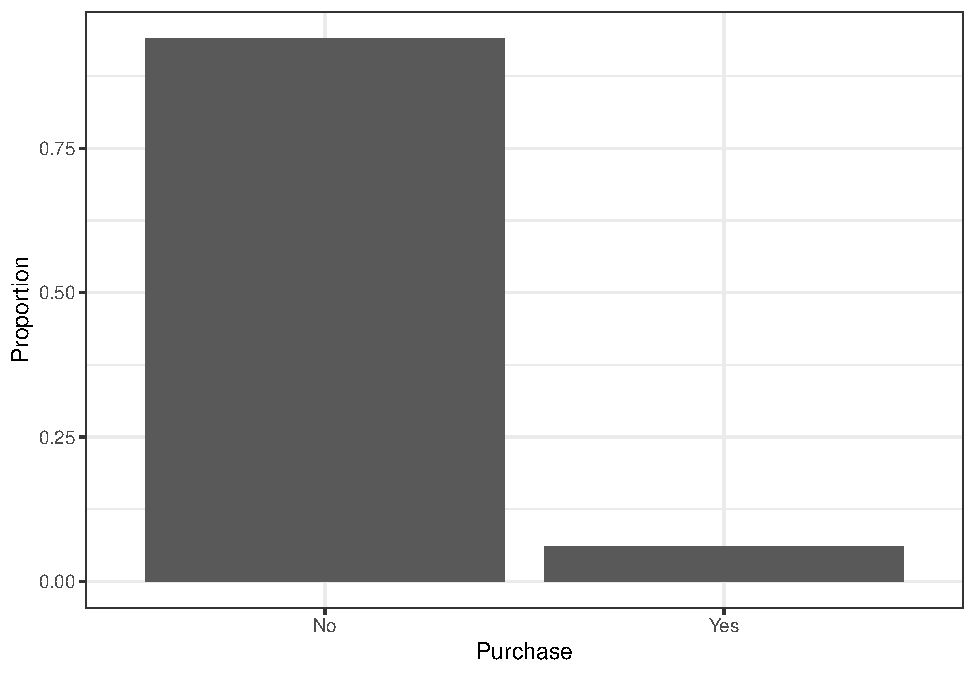
\includegraphics{leroy_francois_hw2_files/figure-latex/unnamed-chunk-5-1.pdf}

\begin{Shaded}
\begin{Highlighting}[]
\KeywordTok{plot}\NormalTok{(}\KeywordTok{dbinom}\NormalTok{(}\DecValTok{1}\OperatorTok{:}\DecValTok{20}\NormalTok{, }\DataTypeTok{size =} \DecValTok{100}\NormalTok{, }\DataTypeTok{prob =} \FloatTok{.06}\NormalTok{))}
\end{Highlighting}
\end{Shaded}

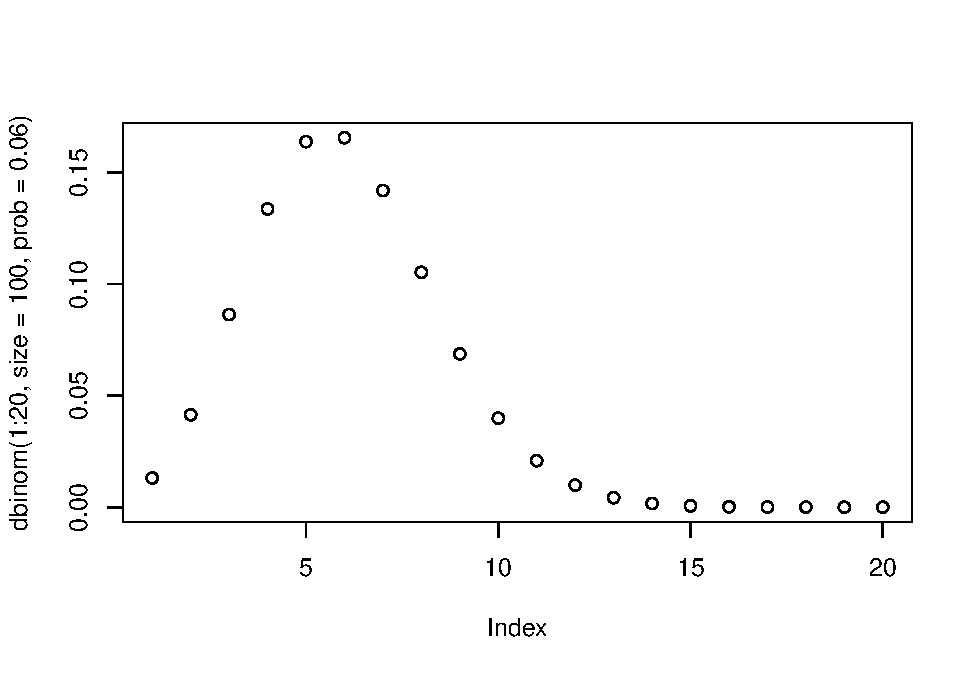
\includegraphics{leroy_francois_hw2_files/figure-latex/unnamed-chunk-6-1.pdf}

We can see that there is 94\% of customers who didn't purchase the insurance and that 6\% who did. As the precision is the number of examples classified as \emph{Yes} when the value is actually \emph{Yes}, by chance, the precision should be 0.06.

\begin{itemize}
\tightlist
\item
  \textbf{1.a. Focus on the customer type MOSHOOFD: create a table with the number of customers that belong to each of 10 L2 groups and the percentage of customers that purchased a caravan insurance policy in each group. Comment the figures in the table. Then do the same for the customer subtype MOSTYPE (41 subgroups defined in L1).}
\end{itemize}

\underline{MOSHOOFD type:}

\begin{Shaded}
\begin{Highlighting}[]
\NormalTok{Caravan }\OperatorTok\StringTok{ }
\StringTok{  }\KeywordTok{count}\NormalTok{(MOSHOOFD, Purchase) }\OperatorTok\StringTok{ }
\StringTok{  }\KeywordTok{group_by}\NormalTok{(MOSHOOFD) }\OperatorTok\StringTok{ }
\StringTok{  }\KeywordTok{summarise}\NormalTok{(}\DataTypeTok{size =} \KeywordTok{sum}\NormalTok{(n),}
            \DataTypeTok{purchase_prop =} \KeywordTok{round}\NormalTok{(n[Purchase }\OperatorTok{==}\StringTok{ "Yes"}\NormalTok{]}\OperatorTok{/}\KeywordTok{sum}\NormalTok{(n), }\DecValTok{2}\NormalTok{)) }\OperatorTok\StringTok{ }
\StringTok{  }\KeywordTok{rename}\NormalTok{(}\DataTypeTok{group =}\NormalTok{ MOSHOOFD) }\OperatorTok\StringTok{ }
\StringTok{  }\NormalTok{kableExtra}\OperatorTok{::}\KeywordTok{kable}\NormalTok{()}
\end{Highlighting}
\end{Shaded}

\begin{tabular}{r|r|r}
\hline
group & size & purchase\_prop\\
\hline
1 & 552 & 0.09\\
\hline
2 & 502 & 0.13\\
\hline
3 & 886 & 0.07\\
\hline
5 & 569 & 0.03\\
\hline
6 & 205 & 0.02\\
\hline
7 & 550 & 0.04\\
\hline
8 & 1563 & 0.06\\
\hline
9 & 667 & 0.06\\
\hline
10 & 276 & 0.02\\
\hline
\end{tabular}

From this first table, we can see that the customers that are more prone to purchase an insurance (13\% of them) are the one belonging to the group 2, \emph{i.e.} the \emph{driven growers}. On the other hand, the customers belonging to the class 6 and 10, respectively the \emph{cruising seniors} and the \emph{farmers}, are less likely to subscribe to the insurance (only 2\% in each group).

\underline{MOSHOOFD type:}

\begin{Shaded}
\begin{Highlighting}[]
\NormalTok{table <-}\StringTok{ }
\NormalTok{Caravan }\OperatorTok\StringTok{ }
\StringTok{  }\KeywordTok{count}\NormalTok{(MOSTYPE, Purchase) }\OperatorTok\StringTok{ }
\StringTok{  }\KeywordTok{group_by}\NormalTok{(MOSTYPE) }\OperatorTok\StringTok{ }
\StringTok{  }\KeywordTok{summarise}\NormalTok{(}\DataTypeTok{size =} \KeywordTok{sum}\NormalTok{(n),}
            \DataTypeTok{purchase_prop =} \KeywordTok{round}\NormalTok{(n[Purchase }\OperatorTok{==}\StringTok{ "Yes"}\NormalTok{]}\OperatorTok{/}\KeywordTok{sum}\NormalTok{(n), }\DecValTok{2}\NormalTok{)) }\OperatorTok\StringTok{ }
\StringTok{  }\KeywordTok{rename}\NormalTok{(}\DataTypeTok{group =}\NormalTok{ MOSTYPE) }\OperatorTok\StringTok{ }
\StringTok{  }\KeywordTok{arrange}\NormalTok{(}\KeywordTok{desc}\NormalTok{(purchase_prop))}
\CommentTok{## Display in 2 columns}
\NormalTok{kableExtra}\OperatorTok{::}\KeywordTok{kable}\NormalTok{(}\KeywordTok{list}\NormalTok{(table[}\DecValTok{1}\OperatorTok{:}\NormalTok{(}\KeywordTok{nrow}\NormalTok{(table)}\OperatorTok{/}\DecValTok{2}\NormalTok{),], }
\NormalTok{                       table[((}\KeywordTok{nrow}\NormalTok{(table)}\OperatorTok{/}\DecValTok{2}\NormalTok{)}\OperatorTok{+}\DecValTok{1}\NormalTok{)}\OperatorTok{:}\KeywordTok{nrow}\NormalTok{(table),])) }\OperatorTok\StringTok{ }
\StringTok{  }\NormalTok{kableExtra}\OperatorTok{::}\KeywordTok{kable_styling}\NormalTok{(}\DataTypeTok{latex_options =} \StringTok{"HOLD_position"}\NormalTok{)}
\end{Highlighting}
\end{Shaded}

\begin{table}[H]

\centering
\begin{tabular}[t]{r|r|r}
\hline
group & size & purchase\_prop\\
\hline
8 & 339 & 0.15\\
\hline
12 & 111 & 0.14\\
\hline
1 & 124 & 0.10\\
\hline
3 & 249 & 0.10\\
\hline
6 & 119 & 0.10\\
\hline
20 & 25 & 0.08\\
\hline
37 & 132 & 0.08\\
\hline
2 & 82 & 0.07\\
\hline
7 & 44 & 0.07\\
\hline
13 & 179 & 0.07\\
\hline
36 & 225 & 0.07\\
\hline
38 & 339 & 0.07\\
\hline
11 & 153 & 0.06\\
\hline
32 & 141 & 0.06\\
\hline
33 & 810 & 0.06\\
\hline
39 & 328 & 0.06\\
\hline
\end{tabular}
\centering
\begin{tabular}[t]{r|r|r}
\hline
group & size & purchase\_prop\\
\hline
10 & 165 & 0.05\\
\hline
34 & 182 & 0.05\\
\hline
4 & 52 & 0.04\\
\hline
5 & 45 & 0.04\\
\hline
9 & 278 & 0.04\\
\hline
22 & 98 & 0.04\\
\hline
35 & 214 & 0.04\\
\hline
24 & 180 & 0.03\\
\hline
30 & 118 & 0.03\\
\hline
31 & 205 & 0.03\\
\hline
23 & 251 & 0.02\\
\hline
25 & 82 & 0.02\\
\hline
26 & 48 & 0.02\\
\hline
27 & 50 & 0.02\\
\hline
29 & 86 & 0.02\\
\hline
41 & 205 & 0.02\\
\hline
\end{tabular}
\end{table}

The two groups more prone to buy an insurance are the group 8 and 12, which correspond respectively to \emph{middle class families} and \emph{affluent young families}. Thus, we can say that families are potential good targets to sell insurances. We can see that the class 25, 26, 27 and 29 all have a low proportion of individuals buying a insurance. They are all related to old people (\emph{i.e.}, \emph{Young seniors in the city}, \emph{Own home elderly}, \emph{Seniors in apartments}, \emph{Porchless seniors: no front yard}). Thus, old people are not a good target to sell insurances.

\textbf{1.b. Analyze the relationship between features MOSHOOFD and MOSTYPE.}

\begin{Shaded}
\begin{Highlighting}[]
\NormalTok{Caravan }\OperatorTok\StringTok{ }
\StringTok{  }\KeywordTok{ggplot}\NormalTok{(}\KeywordTok{aes}\NormalTok{(}\DataTypeTok{y =}\NormalTok{ MOSTYPE, }\DataTypeTok{x =}\NormalTok{ MOSHOOFD))}\OperatorTok{+}
\StringTok{  }\KeywordTok{geom_point}\NormalTok{()}\OperatorTok{+}
\StringTok{  }\KeywordTok{geom_smooth}\NormalTok{(}\DataTypeTok{method =} \StringTok{"lm"}\NormalTok{)}\OperatorTok{+}
\StringTok{  }\KeywordTok{theme_bw}\NormalTok{()}
\end{Highlighting}
\end{Shaded}

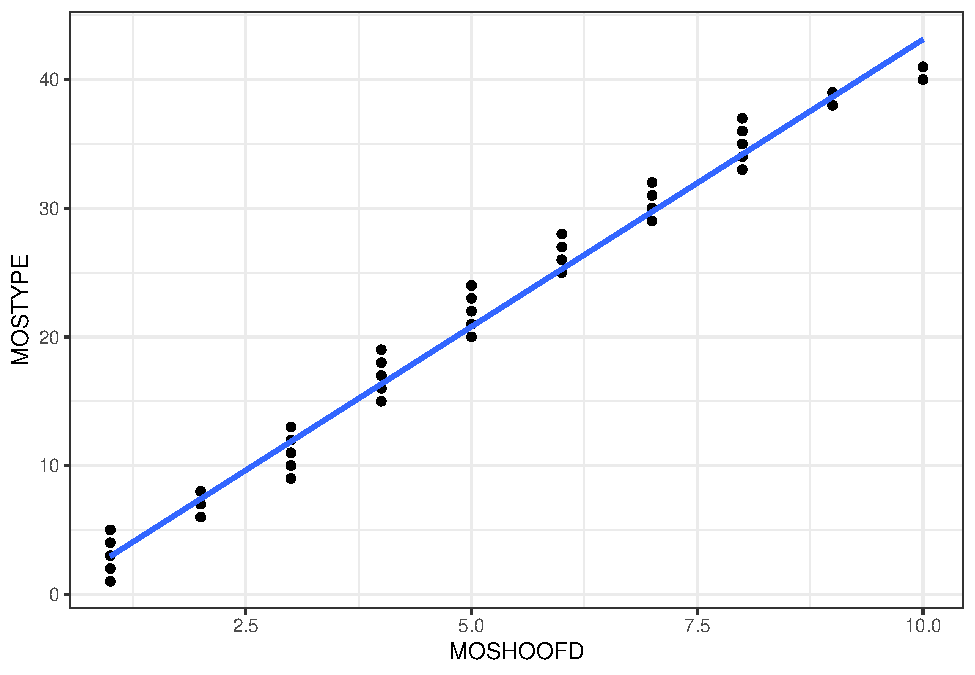
\includegraphics{leroy_francois_hw2_files/figure-latex/unnamed-chunk-9-1.pdf}

We can clearly see a relationship between these two features which are MOSHOOFD = \emph{Customer main type} and MOSTYPE = \emph{Customer Subtype}. This is expected because MOSTYPE is just a more precise social position. For instance, we can see that when \(MOSHOOFD = 10\), \(MOSTYPE = 40 | 41\). We can see that \(MOSHOOFD = 10\) correspond to \emph{Farmers} and that \(MOSTYPE = 40 | 41\) are two subclasses of farmers: \emph{Large family farms} and \emph{Mixed rurals}, respectively.

\hypertarget{task-2---model-fitting-optimization-and-selection}{%
\chapter{Task 2 - Model fitting, optimization, and selection}\label{task-2---model-fitting-optimization-and-selection}}

\begin{Shaded}
\begin{Highlighting}[]
\CommentTok{## Function to randomly extract the test dataset in d_train }
\CommentTok{## using always the same number of positive and negative }
\CommentTok{## values of Purchase}
\NormalTok{prepare_cv_folds <-}\StringTok{  }\ControlFlowTok{function}\NormalTok{(k)\{}
  \CommentTok{# Create the subsets data containing Purchase == Yes }
  \CommentTok{# in one hand and Purchase == No in an other hand}
\NormalTok{  pos_data <-}\StringTok{ }\NormalTok{d_train[d_train}\OperatorTok{$}\NormalTok{Purchase }\OperatorTok{==}\StringTok{ "Yes"}\NormalTok{,]}
\NormalTok{  neg_data <-}\StringTok{ }\NormalTok{d_train[d_train}\OperatorTok{$}\NormalTok{Purchase }\OperatorTok{==}\StringTok{ "No"}\NormalTok{,]}
  \CommentTok{## Compute the size of each fold}
\NormalTok{  fold.size.pos <-}\StringTok{ }\KeywordTok{nrow}\NormalTok{(pos_data)}\OperatorTok\NormalTok{k}
\NormalTok{  fold.size.neg <-}\StringTok{ }\KeywordTok{nrow}\NormalTok{(neg_data)}\OperatorTok\NormalTok{k}
  \CommentTok{## Randomly rearrange the indexes}
  \KeywordTok{set.seed}\NormalTok{(}\DecValTok{12}\NormalTok{); s_pos <-}\StringTok{ }\KeywordTok{sample}\NormalTok{(}\KeywordTok{nrow}\NormalTok{(pos_data))}
  \KeywordTok{set.seed}\NormalTok{(}\DecValTok{12}\NormalTok{); s_neg <-}\StringTok{ }\KeywordTok{sample}\NormalTok{(}\KeywordTok{nrow}\NormalTok{(neg_data))}
  \CommentTok{## create the list that will contain the test folds}
\NormalTok{  f.idx <-}\StringTok{  }\KeywordTok{list}\NormalTok{()}
  \CommentTok{## For each fold, extract the dataset that will be used as test}
  \ControlFlowTok{for}\NormalTok{(i }\ControlFlowTok{in} \DecValTok{1}\OperatorTok{:}\NormalTok{k)\{}
\NormalTok{      f.idx[[i]] <-}\StringTok{ }
\StringTok{        }\KeywordTok{rbind}\NormalTok{(pos_data[s_pos[(}\DecValTok{1} \OperatorTok{+}\StringTok{ }\NormalTok{(i}\DecValTok{-1}\NormalTok{)}\OperatorTok{*}\NormalTok{fold.size.pos)}\OperatorTok{:}\NormalTok{(i}\OperatorTok{*}\NormalTok{fold.size.pos)],],}
\NormalTok{              neg_data[s_neg[(}\DecValTok{1} \OperatorTok{+}\StringTok{ }\NormalTok{(i}\DecValTok{-1}\NormalTok{)}\OperatorTok{*}\NormalTok{fold.size.neg)}\OperatorTok{:}\NormalTok{(i}\OperatorTok{*}\NormalTok{fold.size.neg)],])}
\NormalTok{  \}}
  \KeywordTok{return}\NormalTok{(f.idx)}
\NormalTok{\}}
\CommentTok{## Use the function to create the 10 test datasets}
\NormalTok{split_data <-}\StringTok{ }\KeywordTok{prepare_cv_folds}\NormalTok{(}\DecValTok{10}\NormalTok{)}
\end{Highlighting}
\end{Shaded}

\hypertarget{decision-tree}{%
\section{Decision tree}\label{decision-tree}}

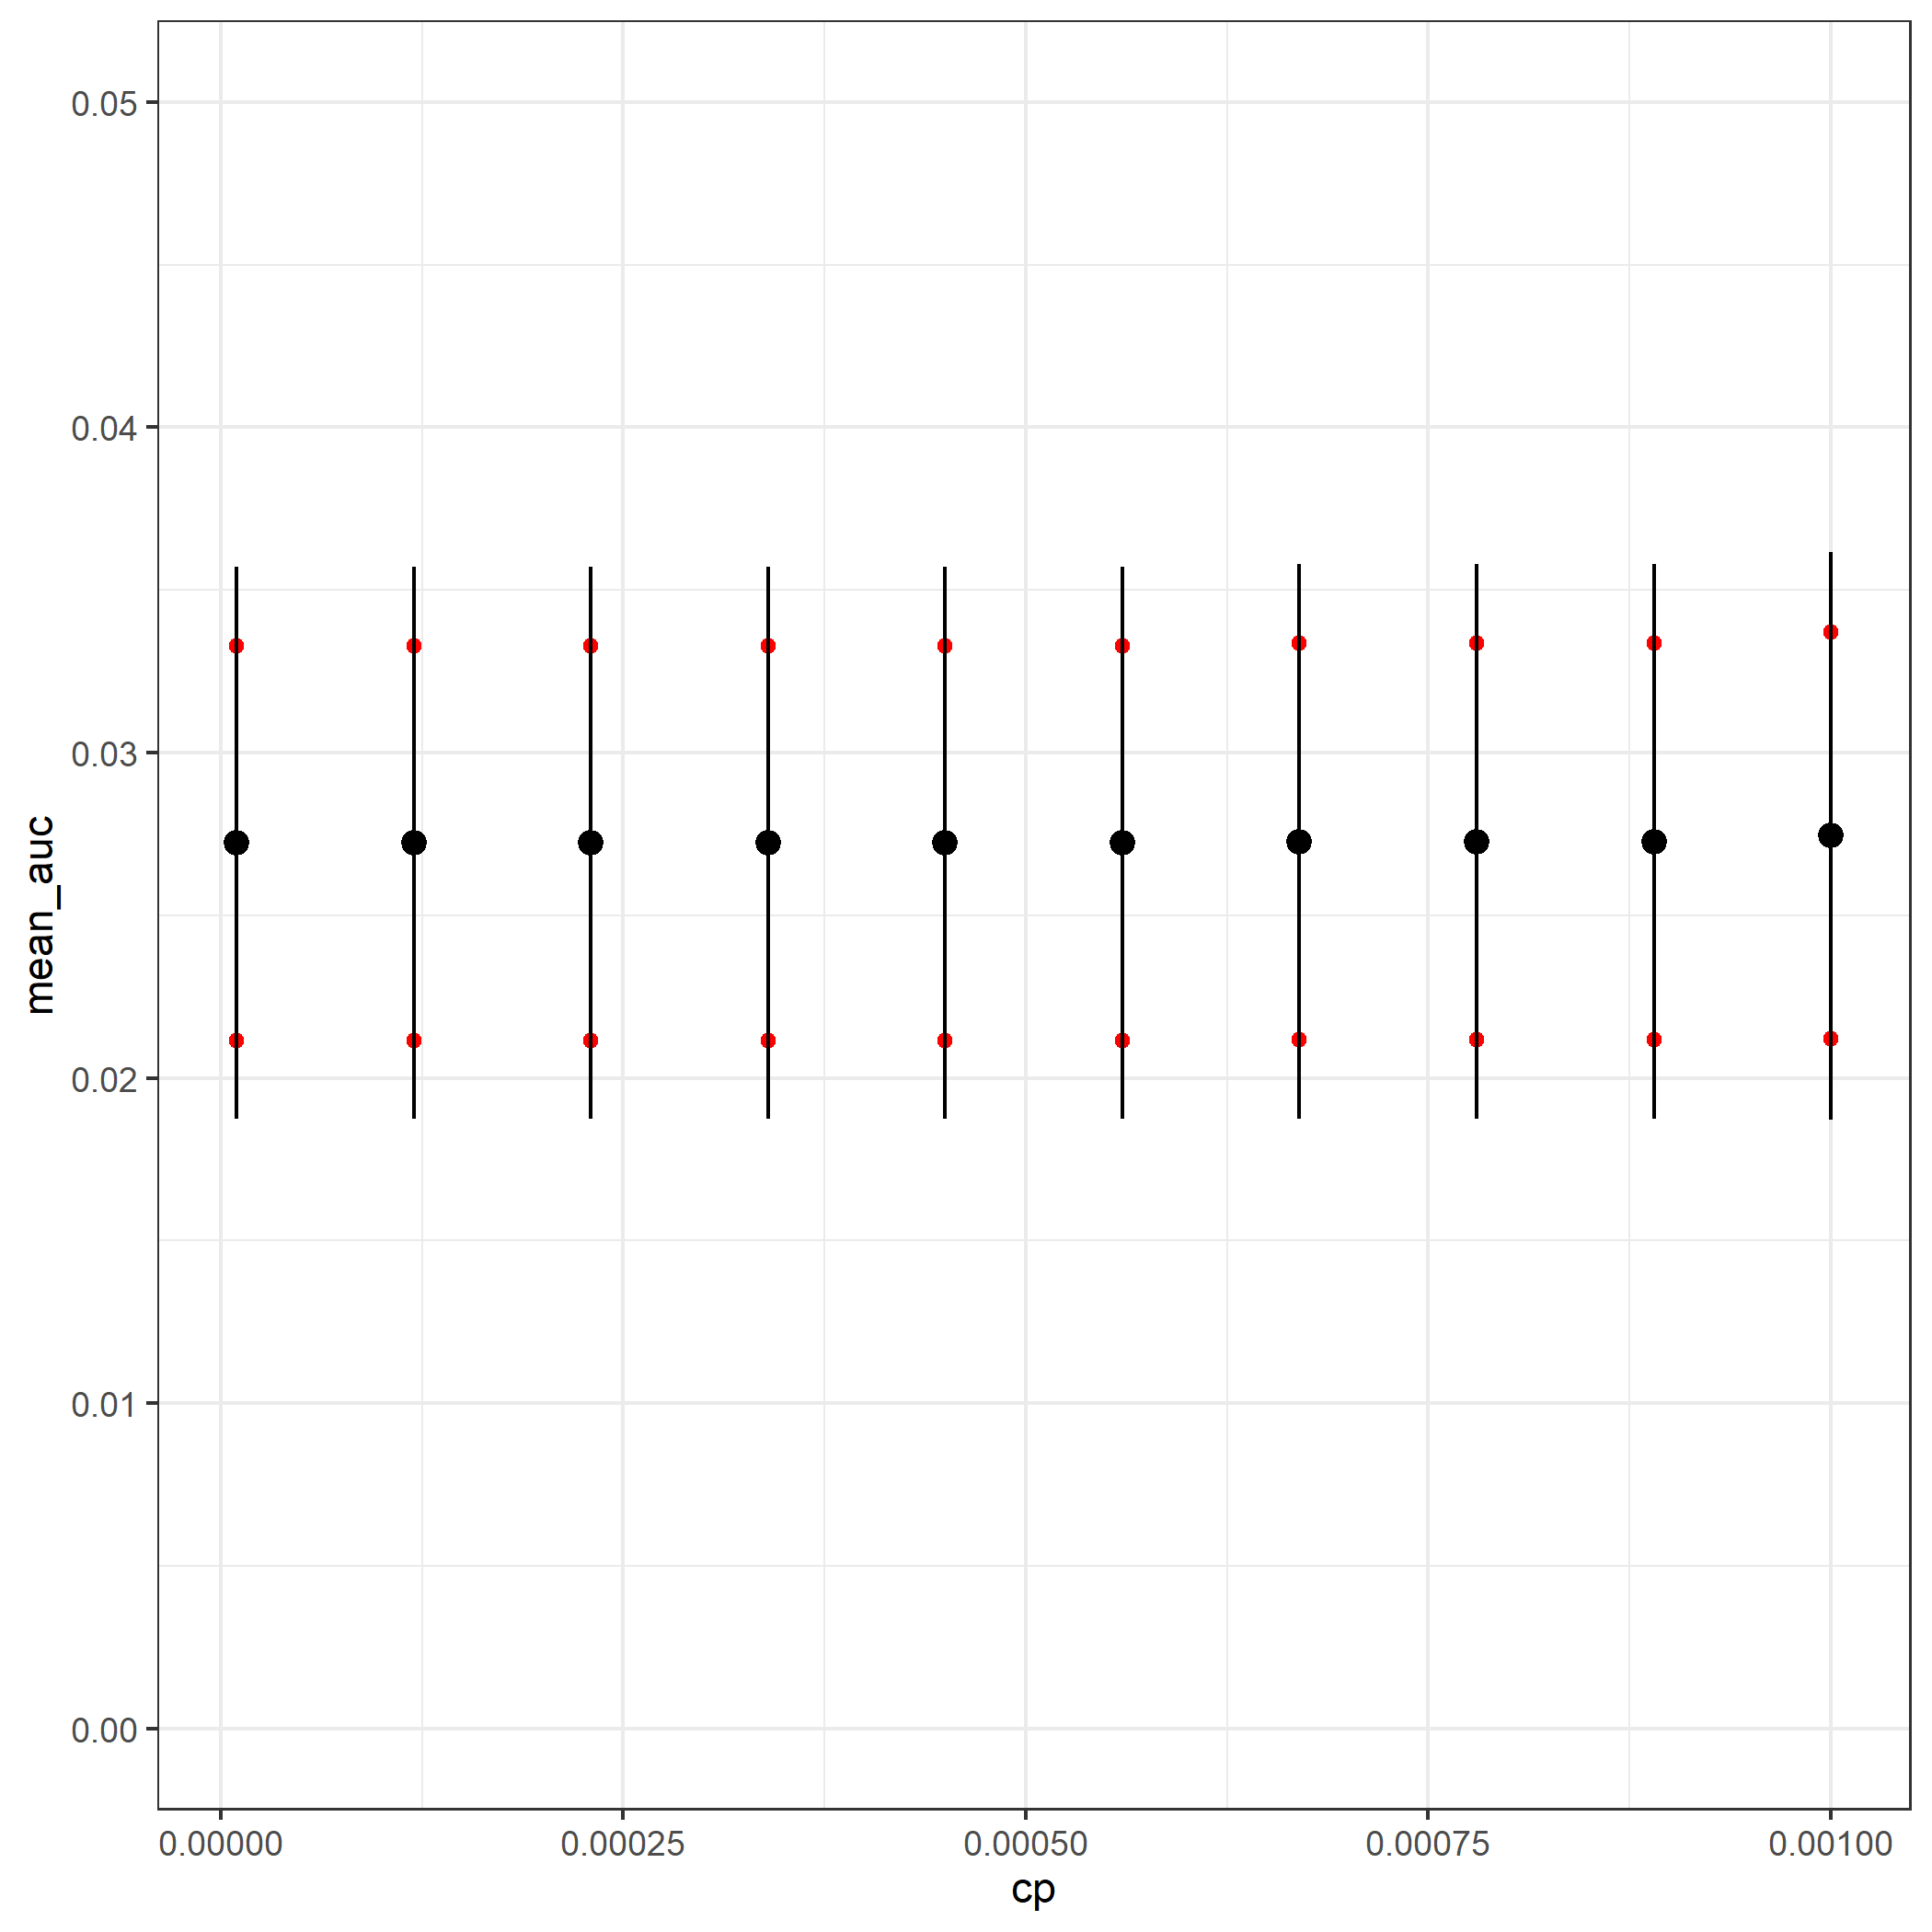
\includegraphics[width=30.15in]{data/cv_dt}

The graphique above shows the mean AUC as a function of different values of cp.~The black lines represent the standard deviation and the red dots the Confidence Intervals. As we can see on this plot, reducing the complexity parameter below \(cp = 0.001\) doesn't change the mean \(AUC_{0.2}\). This means that \(cp = 0.001\) is already sufficiently low. As a low cp means a more complex model, we are looking for the highest value of cp maximizing the mean AUC. Thus, we can select \(cp = 0.001\) to learn the decision tree.

However, as we can see, the mean AUC is always equal to 0.027, which is rather disappointing.

\hypertarget{random-forest}{%
\section{Random Forest}\label{random-forest}}

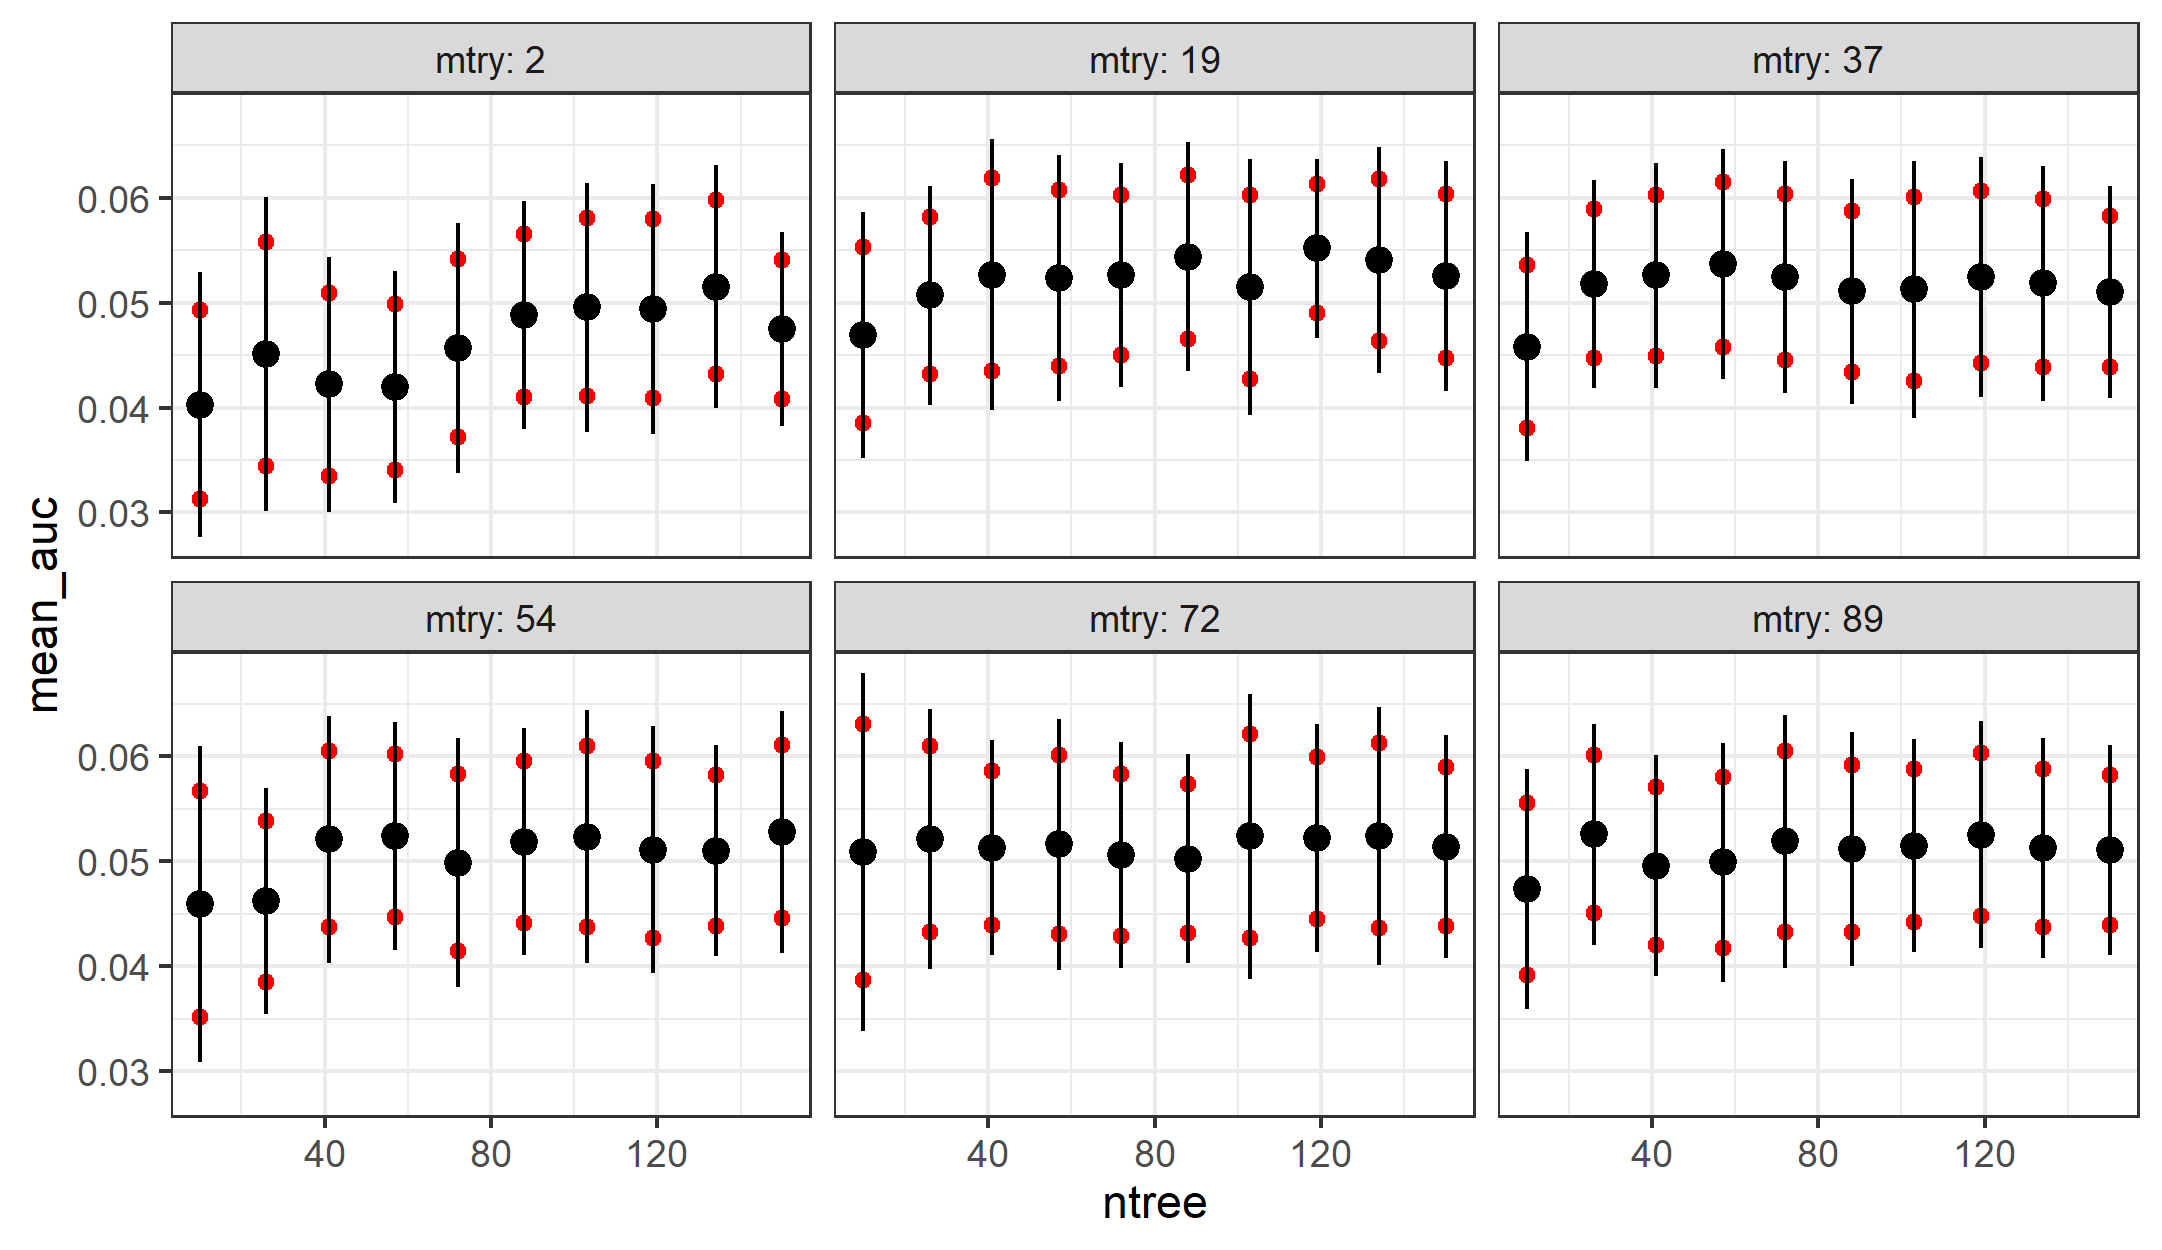
\includegraphics[width=30.03in]{data/cv_rf}

This plot shows the mean auc as a function of the number of trees. Each square correspond to a value of mtry indicated in the grey square. As we can see, the highest value of \(AUC_{0.2}\) is for \(mtry = 72\) and \(ntree = 10\).

However, we must keep in mind that the Confidence Intervals always overlap, which means that the difference between the mean \(AUC_{0.2}\) are not significant.

\hypertarget{regularized-logistic-regression}{%
\section{Regularized logistic regression}\label{regularized-logistic-regression}}

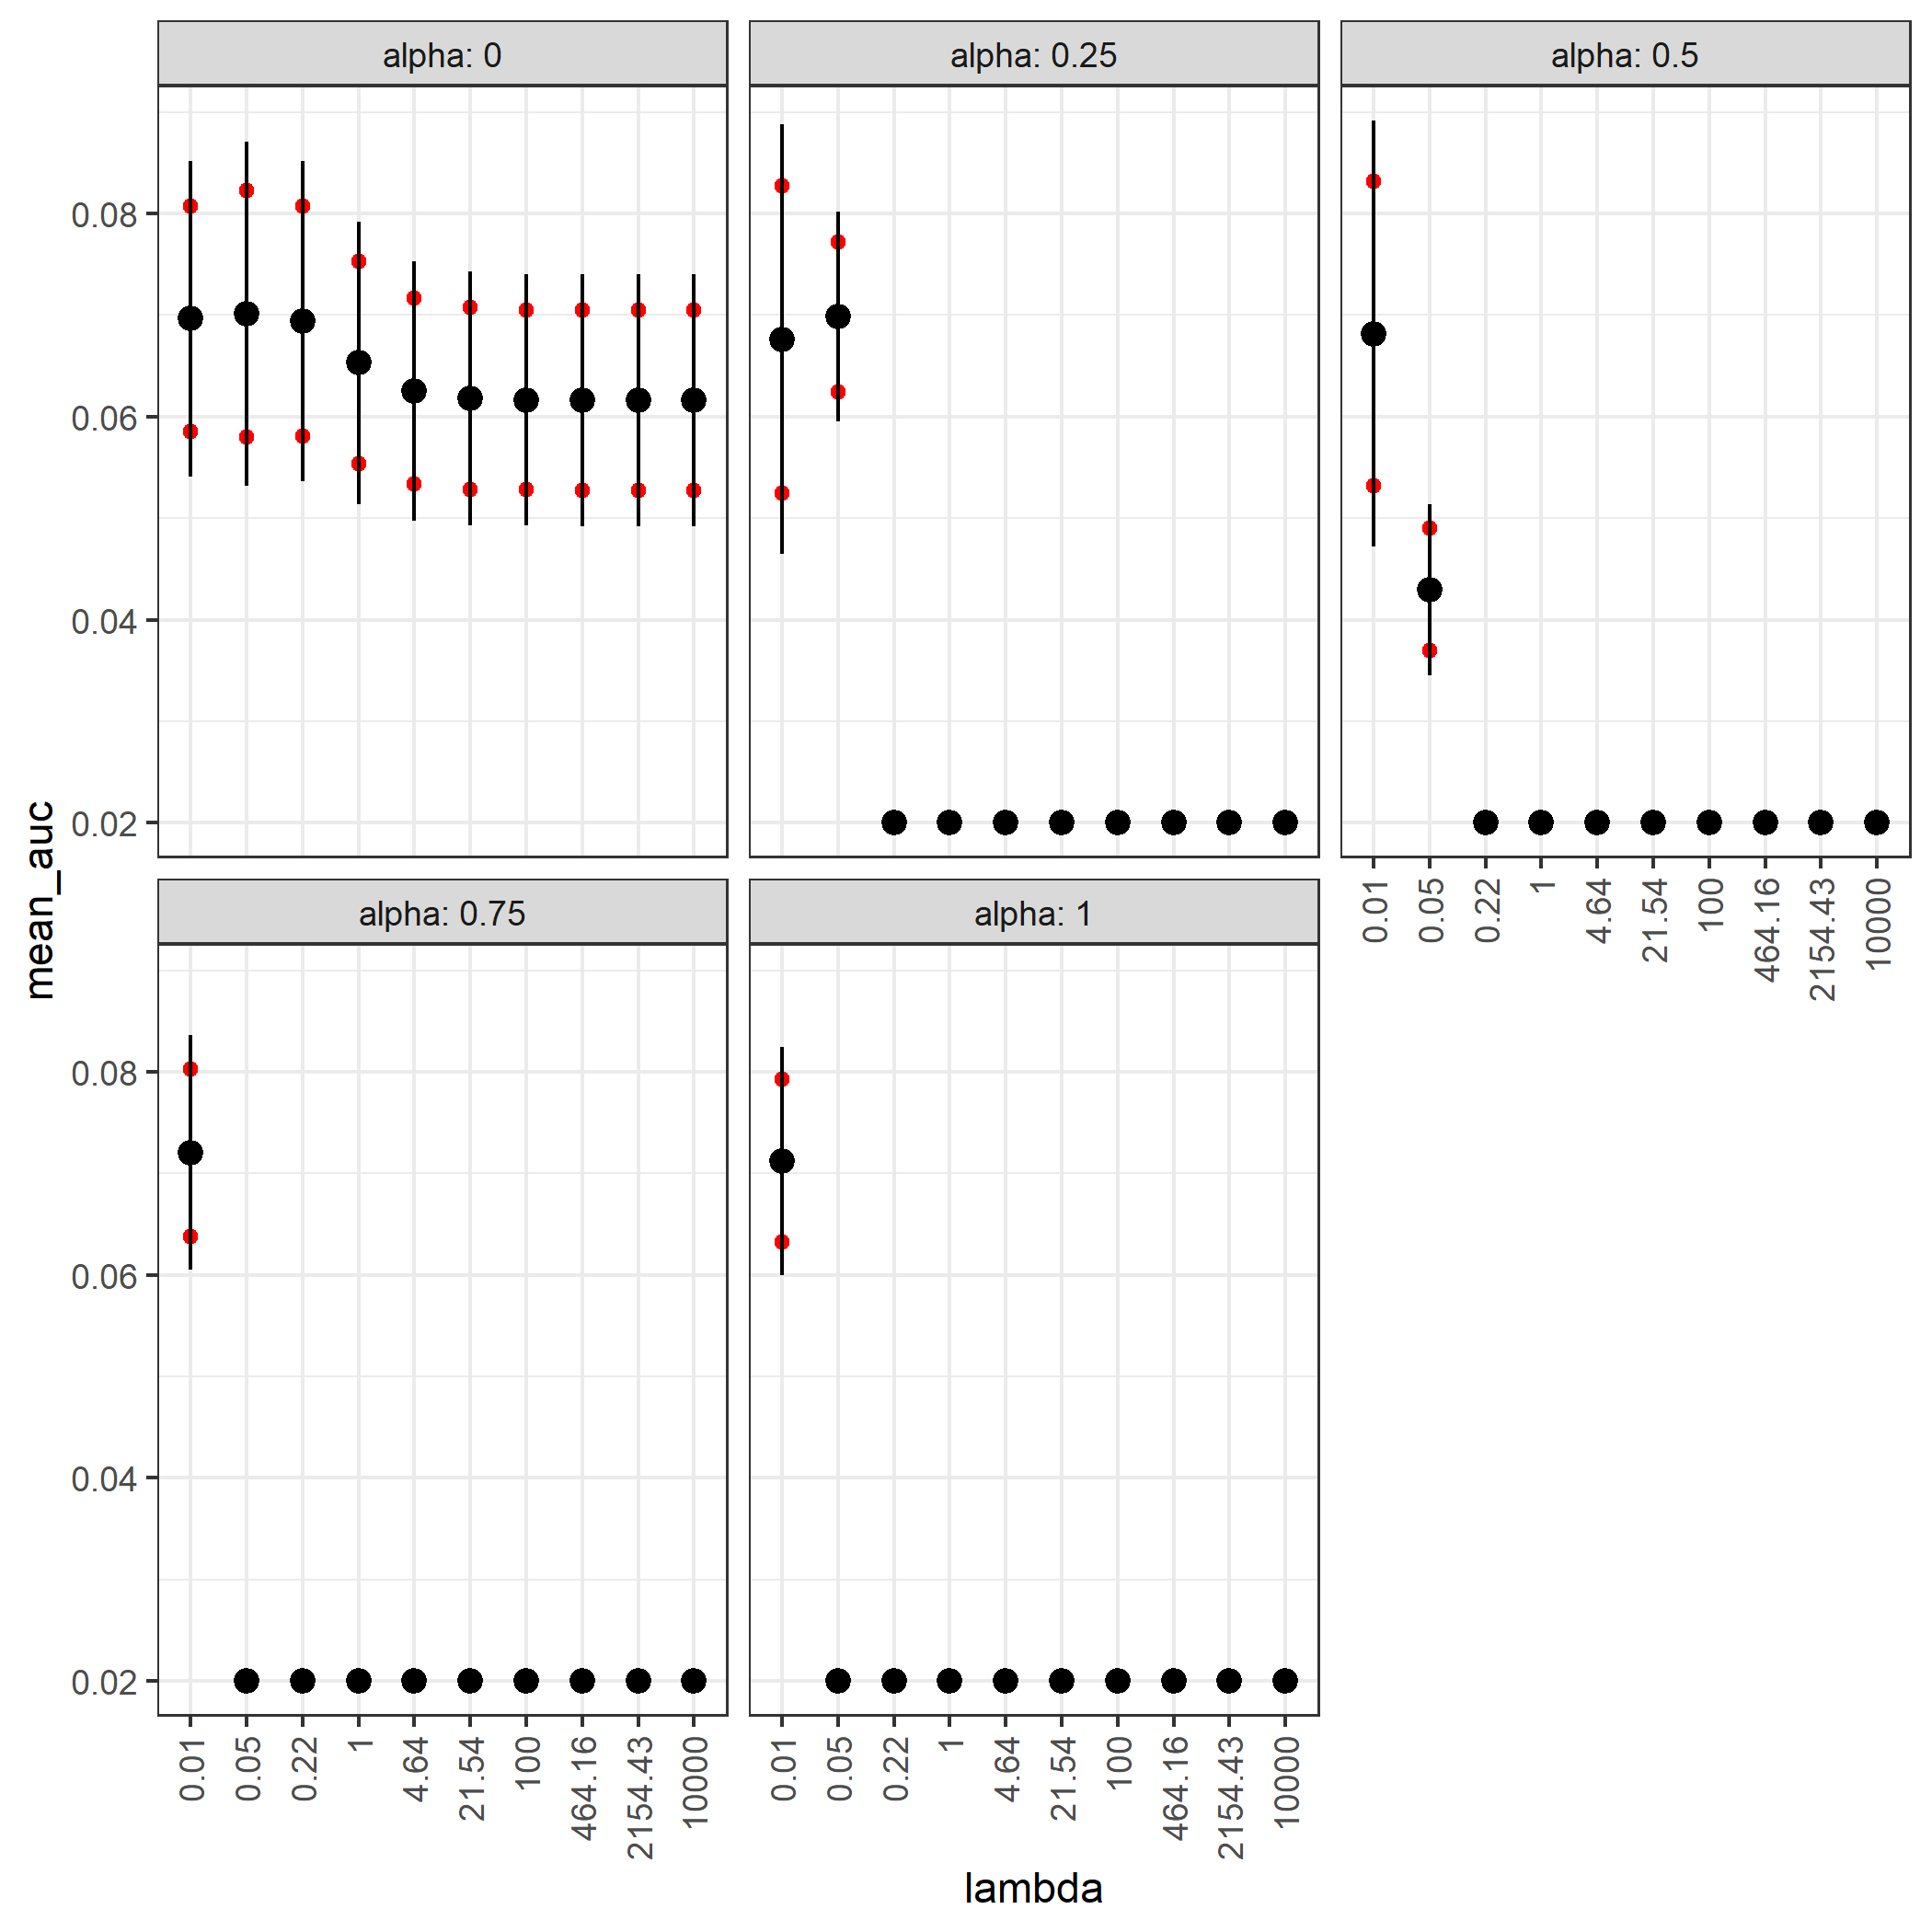
\includegraphics[width=29.17in]{data/cv_lr}

\hypertarget{evaluation-on-the-test-dataset}{%
\section{Evaluation on the test dataset}\label{evaluation-on-the-test-dataset}}

Thanks to the previous steps, we have chosen:

\begin{enumerate}
\def\labelenumi{\arabic{enumi}.}
\item
  A decision tree with \(cp = 0.00067\)
\item
  A random forest with \(ntree = 120\) and \(mtry = 19\)
\item
  A regularized logistic regression with \(\lambda = 0.01\) and \(\alpha = 0.25\)
\end{enumerate}

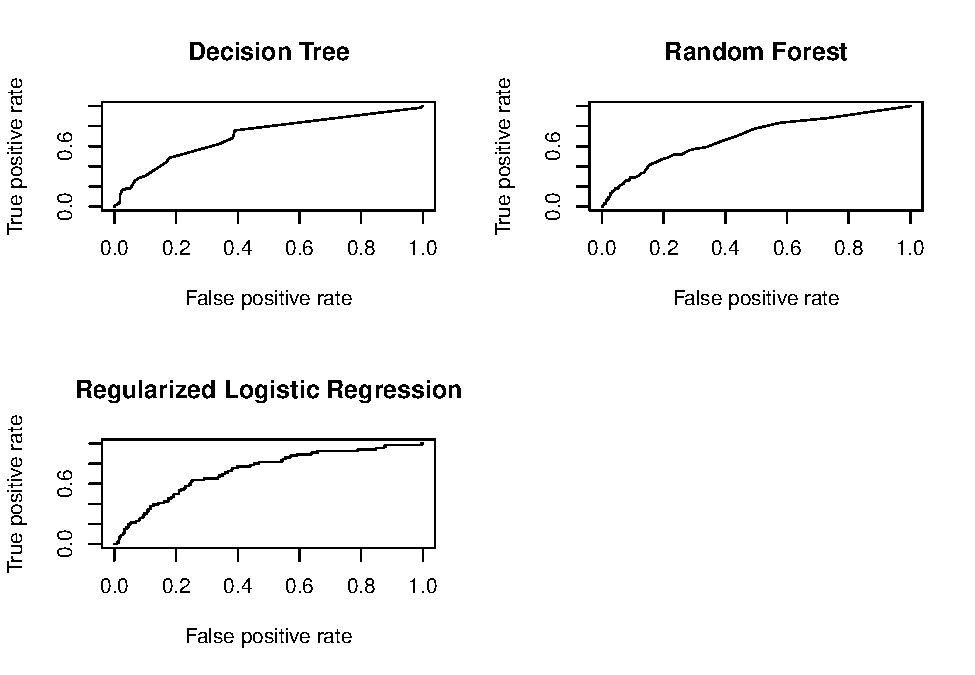
\includegraphics[width=1.5\linewidth]{leroy_francois_hw2_files/figure-latex/unnamed-chunk-17-1}

\begin{table}[H]
\centering
\begin{tabular}{l|r}
\hline
model & auc\\
\hline
Decision Tree & 0.060\\
\hline
Random Forest & 0.055\\
\hline
Regularized Logistic Regression & 0.062\\
\hline
\end{tabular}
\end{table}

\hypertarget{setting-cutoff-threshold}{%
\section{Setting cutoff threshold}\label{setting-cutoff-threshold}}

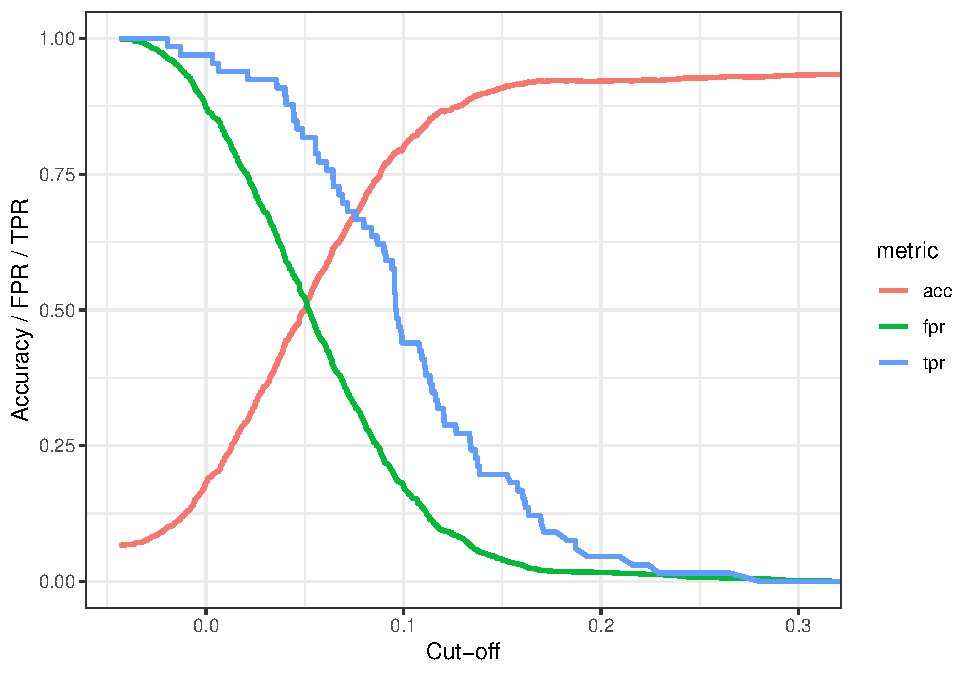
\includegraphics{leroy_francois_hw2_files/figure-latex/unnamed-chunk-19-1.pdf}

The optimal cut-off seems to be \(0.15\) \textbf{1)} because we can see that this is the value where the accuracy is reaching a threshold and \textbf{2)} because this is where the difference between the True Positive Rate and the False Positive Rate is the greatest. This second remark is important because here, we are looking for maximizing the number of true positive while minimizing the number of False Positive.

Now, we can compute the confusion matrix with a threshold of \(0.15\):

\begin{verbatim}
##     obs
## pred   0   1
##    0 897  53
##    1  37  13
\end{verbatim}

\hypertarget{task-3---model-interpretation-and-feature-selection}{%
\chapter{Task 3 - Model interpretation and feature selection}\label{task-3---model-interpretation-and-feature-selection}}

\begin{table}[H]

\centering
\fontsize{9}{11}\selectfont
\begin{tabular}[t]{l|r}
\hline
feature & MeanDecreaseGini\\
\hline
PBRAND & 20.09\\
\hline
MOSTYPE & 17.20\\
\hline
PPERSAUT & 16.73\\
\hline
APERSAUT & 14.74\\
\hline
MKOOPKLA & 11.94\\
\hline
PWAPART & 11.54\\
\hline
MGODGE & 11.08\\
\hline
MBERMIDD & 11.03\\
\hline
MGODPR & 10.97\\
\hline
MOPLMIDD & 10.90\\
\hline
MOSHOOFD & 10.27\\
\hline
MBERARBG & 10.12\\
\hline
MINK3045 & 9.88\\
\hline
MOPLLAAG & 9.86\\
\hline
MFGEKIND & 9.49\\
\hline
MFWEKIND & 9.46\\
\hline
MOPLHOOG & 9.39\\
\hline
MBERARBO & 9.11\\
\hline
MHHUUR & 8.98\\
\hline
MINK4575 & 8.82\\
\hline
MSKB1 & 8.74\\
\hline
MBERHOOG & 8.71\\
\hline
MSKC & 8.31\\
\hline
MHKOOP & 8.27\\
\hline
MINKGEM & 7.92\\
\hline
ABRAND & 7.72\\
\hline
MSKB2 & 7.66\\
\hline
AWAPART & 7.65\\
\hline
\end{tabular}
\centering
\begin{tabular}[t]{l|r}
\hline
feature & MeanDecreaseGini\\
\hline
MINKM30 & 7.55\\
\hline
MSKA & 7.47\\
\hline
MINK7512 & 7.41\\
\hline
MZFONDS & 7.40\\
\hline
MGODOV & 7.33\\
\hline
MFALLEEN & 7.29\\
\hline
MRELGE & 7.20\\
\hline
MAUT1 & 6.95\\
\hline
MZPART & 6.82\\
\hline
MRELOV & 6.26\\
\hline
MAUT0 & 6.18\\
\hline
MAUT2 & 5.99\\
\hline
MGEMLEEF & 5.83\\
\hline
ALEVEN & 5.55\\
\hline
MSKD & 5.39\\
\hline
PLEVEN & 5.07\\
\hline
MGEMOMV & 4.77\\
\hline
MGODRK & 4.72\\
\hline
AFIETS & 4.71\\
\hline
MRELSA & 4.61\\
\hline
MBERZELF & 4.37\\
\hline
PBYSTAND & 3.99\\
\hline
ABYSTAND & 3.73\\
\hline
PPLEZIER & 3.70\\
\hline
APLEZIER & 3.53\\
\hline
MBERBOER & 3.38\\
\hline
PMOTSCO & 3.24\\
\hline
MINK123M & 2.76\\
\hline
\end{tabular}
\centering
\begin{tabular}[t]{l|r}
\hline
feature & MeanDecreaseGini\\
\hline
AMOTSCO & 2.73\\
\hline
PBROM & 2.70\\
\hline
PFIETS & 2.62\\
\hline
ABROM & 2.44\\
\hline
MAANTHUI & 2.43\\
\hline
PWAOREG & 2.36\\
\hline
PGEZONG & 1.65\\
\hline
AWAOREG & 1.59\\
\hline
PTRACTOR & 1.20\\
\hline
PINBOED & 1.15\\
\hline
AGEZONG & 1.11\\
\hline
AINBOED & 1.02\\
\hline
PAANHANG & 0.97\\
\hline
PWABEDR & 0.88\\
\hline
ATRACTOR & 0.78\\
\hline
AWABEDR & 0.73\\
\hline
AAANHANG & 0.69\\
\hline
PBESAUT & 0.49\\
\hline
ABESAUT & 0.47\\
\hline
AZEILPL & 0.27\\
\hline
APERSONG & 0.25\\
\hline
PZEILPL & 0.22\\
\hline
AWALAND & 0.19\\
\hline
PPERSONG & 0.17\\
\hline
PWALAND & 0.15\\
\hline
PWERKT & 0.04\\
\hline
PVRAAUT & 0.01\\
\hline
AWERKT & 0.01\\
\hline
AVRAAUT & 0.00\\
\hline
\end{tabular}
\end{table}


\singlespacing % reset the spacing of the bibliography style
\end{document}
